\documentclass[hyperref={pdfpagelabels=true},ucs]{beamer}

%\usetheme{Warsaw}
\usetheme{GSyC}


%\usebackgroundtemplate{
\includegraphics[width=\paperwidth]{../format/blank-bg.png}}


\usepackage[spanish]{babel}
\usepackage[utf8x]{inputenc}
\usepackage{graphics}
\usepackage{amssymb} % Simbolos matematicos
\usepackage{fancyvrb}
\usepackage{multicol}
\usepackage{alltt}
\usepackage{listings}




\definecolor{darkred}{rgb}  {1.0, 0.0, 0.0}
\definecolor{darkgreen}{rgb}{0.0, 0.4, 0.0}
\definecolor{darkblue}{rgb} {0.0, 0.0, 0.8}

% for resalted text
\newcommand{\res}[1]{\textcolor{darkred}{#1}}
% for different text
\newcommand{\dif}{\textsl}
% for reserved words
\newcommand{\rw}[1]{\textrm{\textbf{#1}}}
% for commands
\newcommand{\com}[1]{\textrm{\textbf{#1}}}

% for java code. Usage: \begin{java} java code... \end{java}
\lstnewenvironment{java} 
{\lstset{language=java,numbers=left,stepnumber=2}} 
{} 

% for xml code. Usage: \begin{xml} xml code... \end{xml}
\lstnewenvironment{xml} 
{\lstset{language=xml,numbers=left,stepnumber=2}} 
{} 

\fvset{commandchars=\\\{\},frame=single}



%% Metadatos del PDF.
\hypersetup{
  pdftitle={Curso de Desarrollo en Android},
  pdfauthor={GSyC/LibreSoft},
  pdfcreator={GSyC/LibreSoft},
  pdfproducer=PDFLaTeX,
  pdfsubject={Anatomia y Fundamentos de las Aplicaciones},
}
%%


%\pgfdeclareimage[height=0.5cm]{gsyc-logo}{../format/gsyc}
%\logo{\pgfuseimage{gsyc-logo}}



\AtBeginSection[]
{
  \begin{frame}<beamer>[shrink=20]{Contenidos}
    \tableofcontents[currentsection,hideallsubsections]
  \end{frame}
}

% \AtBeginSubsection[]
% {
%   \begin{frame}<beamer>{Contenidos}
%     \tableofcontents[currentsection,currentsubsection]
%   \end{frame}
% }




\begin{document}

%% Entre corchetes como argumento opcional un título o autor abreviado
%% para los pies de transpa

\title[Anatomia y Fundamentos de las Aplicaciones]{Anatomia y Fundamentos de las Aplicaciones}
\subtitle{Curso de Desarrollo en Android}
%\institute{gsyc-profes@gsyc.escet.urjc.es}
\author[GSyC/LibreSoft]{GSyC/LibreSoft}
\date[2011]{Marzo de 2011}

\frame{
\titlepage
\begin{center}
%\includegraphics[width=2cm]{../format/gsyc}
\end{center}
}




%% LICENCIA DE REDISTRIBUCIÓN DE LAS TRANSPAS
\frame{
~
\vspace{4cm}
\begin{flushright}
{\tiny
\copyright 2011 GSyC/LibreSoft \\
  Algunos derechos reservados. \\
  Este trabajo se distribuye bajo la licencia \\
  Creative Commons Attribution Share-Alike\\
  disponible en http://creativecommons.org/licenses/by-sa/3.0/es\\
}
\end{flushright}
}
%%
%%%%%%%%%%%%%%%%%%%%%%%%%%%%%%%%%%%%%%%%%%%%%%%%%%%%%%%%%%%%%%%%%%%

\begin{frame}[shrink=20]
  \frametitle{Contenidos}
  \tableofcontents[hideallsubsections]
\end{frame}


%%%%%%%%%%%%%%%%%%%%%%%%%%%%%%%%%%%%%%%%%%%%%%%%%%%%%%%%%%%%%%%%%%%
\section{Intenciones (Intents)}
%%%%%%%%%%%%%%%%%%%%%%%%%%%%%%%%%%%%%%%%%%%%%%%%%%%%%%%%%%%%%%%%%%%




%%%%%%%%%%%%%%%%%%%%%%%%%%%%%%%%%%%%%%%%%%%%
\begin{frame}[shrink=15]
\frametitle{Componentes de las Aplicaciones Android}

\begin{itemize}
\item \alert{Actividades \emph{(Activities)}}: Cada pantalla de una aplicación. Utilizan
  \alert{Vistas \emph{(Views)}} como componentes que muestran
  información y responden a las acciones del usuario
\item \alert{Servicios \emph{(Services)}}: Componentes de la
  aplicación que se ejecutan de forma invisible, actualizando los
  datos y las Actividades, y disparando Notificaciones. Realizan el
  procesamiento normal de la aplicación que debe continuar incluso
  cuando las Actividades de la aplicación no están visibles.
\item \alert{Proveedores de Contenidos \emph{(Content Providers)}}:
  Almacenes de datos compartidos. Gestionan las Bases de Datos para las
  aplicaciones.
\item \alert{Intenciones \emph{(Intents)}}: Mecanismo que permite el paso
  de mensajes destinados a ciertas Actividades o Servicios, o a todo
  el sistema (Intenciones de \emph{broadcast}). Exponen la intención de
  que se haga algo. El sistema determinará el destinatario que lo efectuará.
\item \alert{Receptores de \emph{Broadcast} \emph{(Broadcast
      Receivers)}}: Los crean las aplicaciones como consumidores de
  las Intenciones de \emph{broadcast} que cumplan ciertos criterios.
\item \alert{Notificaciones \emph{(Notifications)}}: Mecanismo que
  permite a las aplicaciones señalar algo a los usuarios sin
  interrumpir la Actividad en primer plano.
\end{itemize}

\end{frame}


%%%%%%%%%%%%%%%%%%%%%%%%%%%%%%%%%%%%%%%%%
\begin{frame}[fragile]
\frametitle{El Manifiesto de una Aplicación (I)}  

\begin{itemize}
\item Cada Aplicación incluye un fichero de Manifiesto,
  \Verb|\textcolor{red}{AndroidManifest.xml}|.
\item Define la estructura de la aplicación y sus componentes.
\item Incluye un nodo raíz y un nodo para cada
  uno de sus tipos de componentes.
\item A través de \textbf{filtros de intenciones} y \textbf{permisos}
  determina cómo interactuará con otras aplicaciones.
\item Nodo raíz \Verb|\alert{manifest}|: incluye el nombre del paquete de
  la aplicación:

\begin{tiny}
\begin{block}{}
\begin{xml}
<manifest xmlns:android=http://schemas.android.com/apk/res/android
          package="com.my_domain.my_app">
          [ ... manifest nodes ... ]
</manifest>
\end{xml}
\end{block}
\end{tiny}

\end{itemize}

\end{frame}


%%%%%%%%%%%%%%%%%%%%%%%%%%%%%%%%%%%%%%%%%
\begin{frame}[fragile]
\frametitle{El Manifiesto de una Aplicación (II)}  

\begin{itemize}

\item Nodo \Verb|\alert{application}|:
  \begin{itemize}
  \item Indica metadatos de la aplicación (título, icono, tema)
  \item Contiene los nodos de actividades, servicios, proveedores de
    contenidos y receptores de broadcast.
  \end{itemize}

\begin{tiny}
\begin{block}{}
\begin{xml}
<application android:icon="@drawable/icon"
             android:theme="@style/my_theme">
  <activity android:name=".MyActivity" android:label="@string/app_name">
    <intent-filter>
      <action android:name="android.intent.action.MAIN" />
      <category android:name="android.intent.category.LAUNCHER" />
    </intent-filter>
  </activity>

  <activity ... >
    ...
  </activity>

  <service ... >
    ...
  </service>

  ...

</application>
\end{xml}
\end{block}
\end{tiny}

\end{itemize}

\end{frame}



%%%%%%%%%%%%%%%%%%%%%%%%%%%%%%%%%%%%%%%%%
\begin{frame}[fragile]
\frametitle{El Manifiesto de una Aplicación (III)}  

\begin{itemize}

\item Nodo \Verb|\alert{uses-permission}|:
  \begin{itemize}
  \item Declara los permisos que la aplicación necesita para operar.
  \item Serán presentados al usuario durante la instalación para que
    los acepte o deniegue.
  \item Se requieren permisos para utilizar muchos de los servicios
    nativos Android (enviar SMS, hacer llamadas, usar servicios de
    localización\ldots)
  \item Permisos más habituales:
    \verb|INTERNET, READ_CONTACTS,| \verb|WRITE_CONTACTS,|
    \verb|RECEIVE_SMS, SEND_SMS,| \verb|ACCESS_COARSE_LOCATION,|
    \verb|ACCESS_FINE_LOCATION|
  \end{itemize}

\begin{tiny}
\begin{block}{}
\begin{xml}
<uses-permission android:name="android.permission.ACCESS_FINE_LOCATION">
</uses-permission>
\end{xml}
\end{block}
\end{tiny}

\end{itemize}

\end{frame}



%%%%%%%%%%%%%%%%%%%%%%%%%%%%%%%%%%%%%%%%%
\begin{frame}[fragile]
\frametitle{El Manifiesto de una Aplicación (IV)}  

\begin{itemize}

\item Nodo \Verb|\alert{permission}|:
  \begin{itemize}
  \item Define un permiso que se requiere para que otras aplicaciones
    puedan acceder a partes restringidas de la aplicación
  \item Las otras aplicaciones necesitarán poner un
    \verb|uses-permission| en su Manifiesto para utilizar este permiso
  \end{itemize}

\begin{tiny}
\begin{block}{}
\begin{xml}
<permission android:name="com.clau.DETONATE_DEVICE"
            android:protectionLevel="dangerous"
            android:label="Self Destruct"
            android:description="@string/detonate_description">
</permission>
\end{xml}
\end{block}
\end{tiny}


\end{itemize}

\end{frame}



%%%%%%%%%%%%%%%%%%%%%%%%%%%%%%%%%%%%%%%%%
\begin{frame}[fragile]
\frametitle{El Manifiesto de una Aplicación (V)}  

\begin{itemize}

\item Nodo \Verb|\alert{instrumentation}|:

  \begin{itemize}
  \item Permite definir tests de ejecución para las Actividades
    y Servicios.
  \end{itemize}

\begin{scriptsize}
\begin{block}{}
\begin{xml}
<instrumentation android:label="My Test"
                 android:name=".MyTestClass"
                 android:targetPackage="com.clau.aPackage">
</instrumentation>
\end{xml}
\end{block}
\end{scriptsize}

\item Más información sobre el manifiesto en:\\
  \begin{scriptsize}
    \Verb|http://code.google.com/android/devel/bblocks-manifest.html|
  \end{scriptsize}
\end{itemize}

\end{frame}



%%%%%%%%%%%%%%%%%%%%%%%%%%%%%%%%%%%%%%%%%%%%%%%%%%%%%%%%%%%%%%%%%%%
\section{Creación y destrucción de Aplicaciones y Actividades}
%%%%%%%%%%%%%%%%%%%%%%%%%%%%%%%%%%%%%%%%%%%%%%%%%%%%%%%%%%%%%%%%%%%



%%%%%%%%%%%%%%%%%%%%%%%%%%%%%%%%%%%%%%%%%%%%
\begin{frame}[shrink=15]
\frametitle{Aplicaciones, Actividades y  Pila de Actividades}
  
\begin{itemize}
\item Las Aplicaciones Android no son iguales a las aplicaciones
  en los sistemas operativos tradicionales: sólo hay una en primer
  plano que normalmente ocupa toda la pantalla.
\item Las Aplicaciones están formadas por \alert{Actividades}
  (pantallas).
\item Al arrancar una nueva aplicación, pasa a primer plano situando
  una Actividad encima de la que hubiera, formándose así una
  \textcolor{red}{Pila de Actividades}.
\item El botón \emph{Back} ($\hookleftarrow$) cierra la Actividad en
  primer plano y recupera la de la cima de la Pila (cerrando la
  aplicación en su caso).
\end{itemize}

\begin{center}
  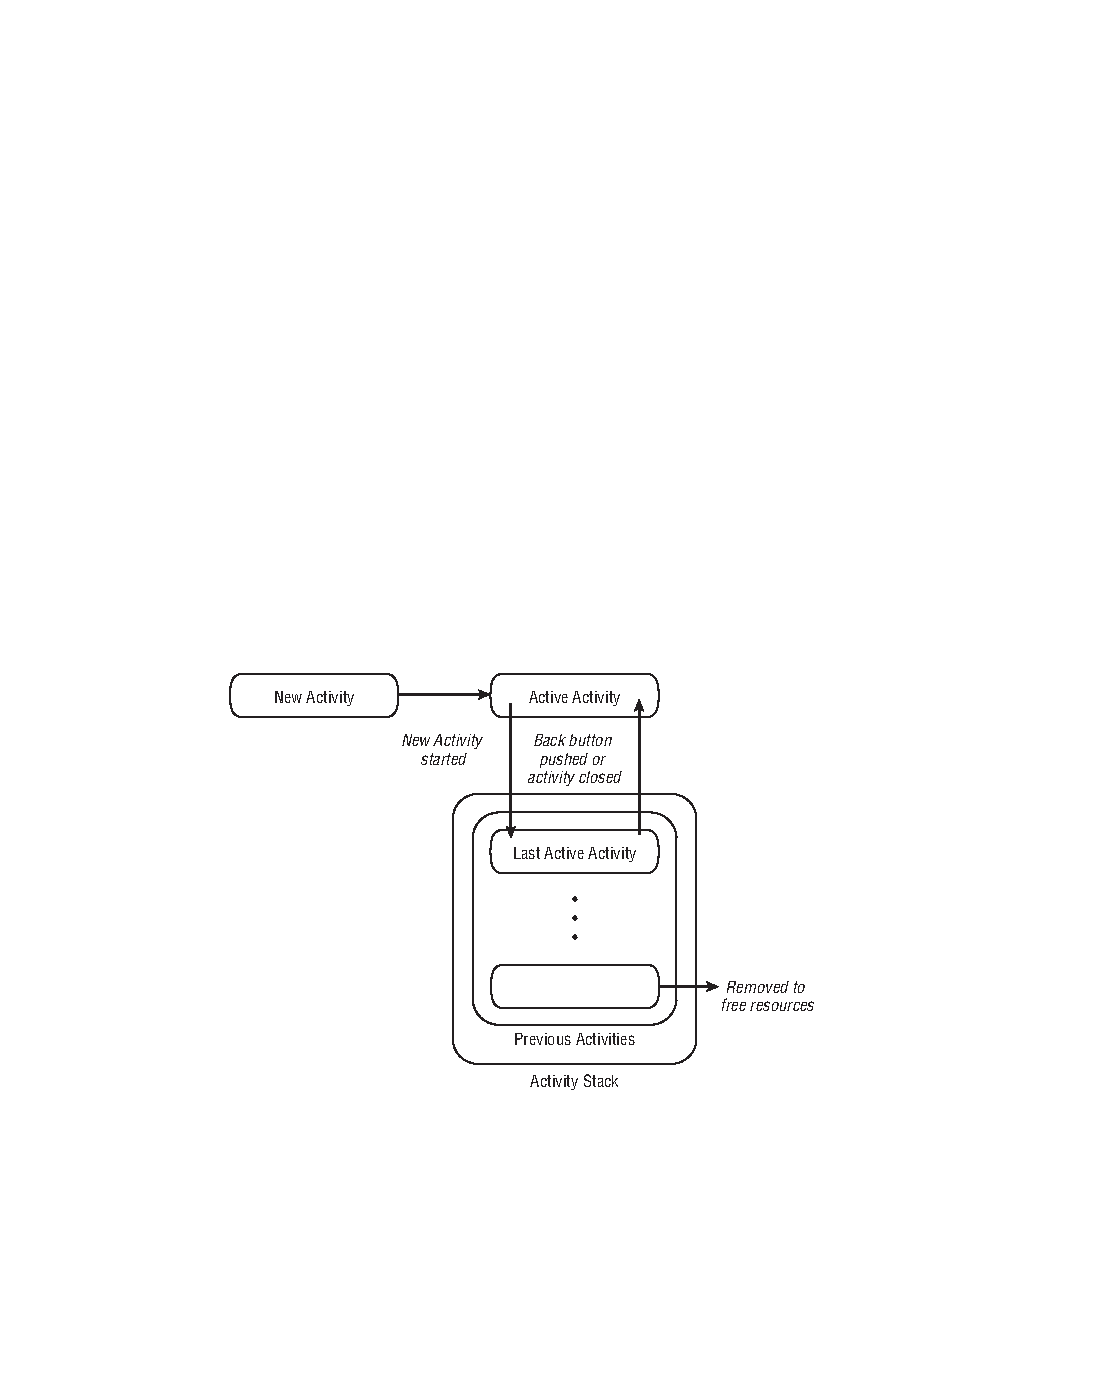
\includegraphics[height=50mm]{figs/PAAD-p68}
\end{center}



\end{frame}



%%%%%%%%%%%%%%%%%%%%%%%%%%%%%%%%%%%%%%%%%%%%
\begin{frame}
\frametitle{Aplicaciones y procesos}

\begin{itemize}
\item Las aplicaciones Android no tienen control sobre su propio
  ciclo de vida:
  \begin{itemize}
  \item deben estar pendientes de posibles cambios en su estado y
    reaccionar como corresponda
  \item en particular, deben estar preparadas para su terminación en
    cualquier momento
  \end{itemize}
\item En general, cada aplicación Android se ejecuta en un proceso que
  ejecuta una instancia de Dalvik.
\item \alert{Android mata sin previo aviso los procesos que considera
  necesarios cuando lo considera necesario para mantener el sistema
  responsivo}.
\item El \emph{runtime} de Android gestiona el proceso de cada
  aplicación, y por extensión de cada Actividad que contenga.

\end{itemize}

\end{frame}



%%%%%%%%%%%%%%%%%%%%%%%%%%%%%%%%%%%%%%%%%%%%
\begin{frame}
\frametitle{Aplicaciones, Actividades, Vistas, Diseños}

\begin{itemize}

\item Una Actividad representa una pantalla que una aplicación muestra
  a sus usuarios (equivalente al concepto de \emph{Form} en
  aplicaciones de escritorio convencionales).

\item La mayoría de las Actividades ocupan toda la pantalla del
  dispositivo, pero pueden crearse actividades semi-transparentes,
  flotantes o que utilizan cajas de diálogo.

\item Para crear una nueva Actividad en una aplicación se hereda de la
  clase \Verb|\alert{Activity}|.

\item Las Interfaz de Usuario de una Actividad se crea mediante
  \alert{Vistas} \emph{(Views)} (equivalentes al concepto de
  \emph{Widgets} en aplicaciones de escritorio convencionales).

\item Las Vistas se agrupan en Diseños \emph{(Layouts)} que mostrará la
  aplicación.

\end{itemize}

\end{frame}



%%%%%%%%%%%%%%%%%%%%%%%%%%%%%%%%%%%%%%%%%%%%
\begin{frame}[fragile,shrink=25]
\frametitle{Creación de una Actividad}

\begin{scriptsize}
\begin{block}{src/com.clau.myapplication/MyActivity.java}
\begin{java}
  package com.clau.myapplication;

  import android.app.Activity; 
  import android.os.Bundle;

  public class MyActivity extends Activity { 
    /** Called when the activity is first created. */ 
    @Override 
    public void onCreate(Bundle savedInstanceState) { 
      super.onCreate(savedInstanceState);
      setContentView(R.layout.main);
    }
  }
\end{java}
\end{block}
\end{scriptsize}

\begin{itemize}
\item Para usar una Actividad en una Aplicación, hay que registrarla
  en el \alert{Manifiesto}, incluyendo las Intenciones a las que responderá:
\begin{scriptsize}
\begin{block}{AndroidManifest.xml}
\begin{xml}
<activity android:label="@string/app_name"
          android:name=".MyActivity">
  <intent-filter>
    <action android:name="android.intent.action.MAIN" />
    <category android:name="android.intent.category.LAUNCHER" />
  </intent-filter>
</activity>
\end{xml}
\end{block}
\end{scriptsize}

\end{itemize}


\end{frame}


%%%%%%%%%%%%%%%%%%%%%%%%%%%%%%%%%%%%%%%%%%%%
\begin{frame}[shrink=30]
\frametitle{Procesos y prioridades}

\begin{itemize}
\item El orden en que los procesos se van matando para liberar
  recursos lo determina las prioridades de la aplicaciones que alojan.
\item Árbol de prioridades:

\end{itemize}

  \begin{columns}[c]


\column{52mm}

    \begin{center}
      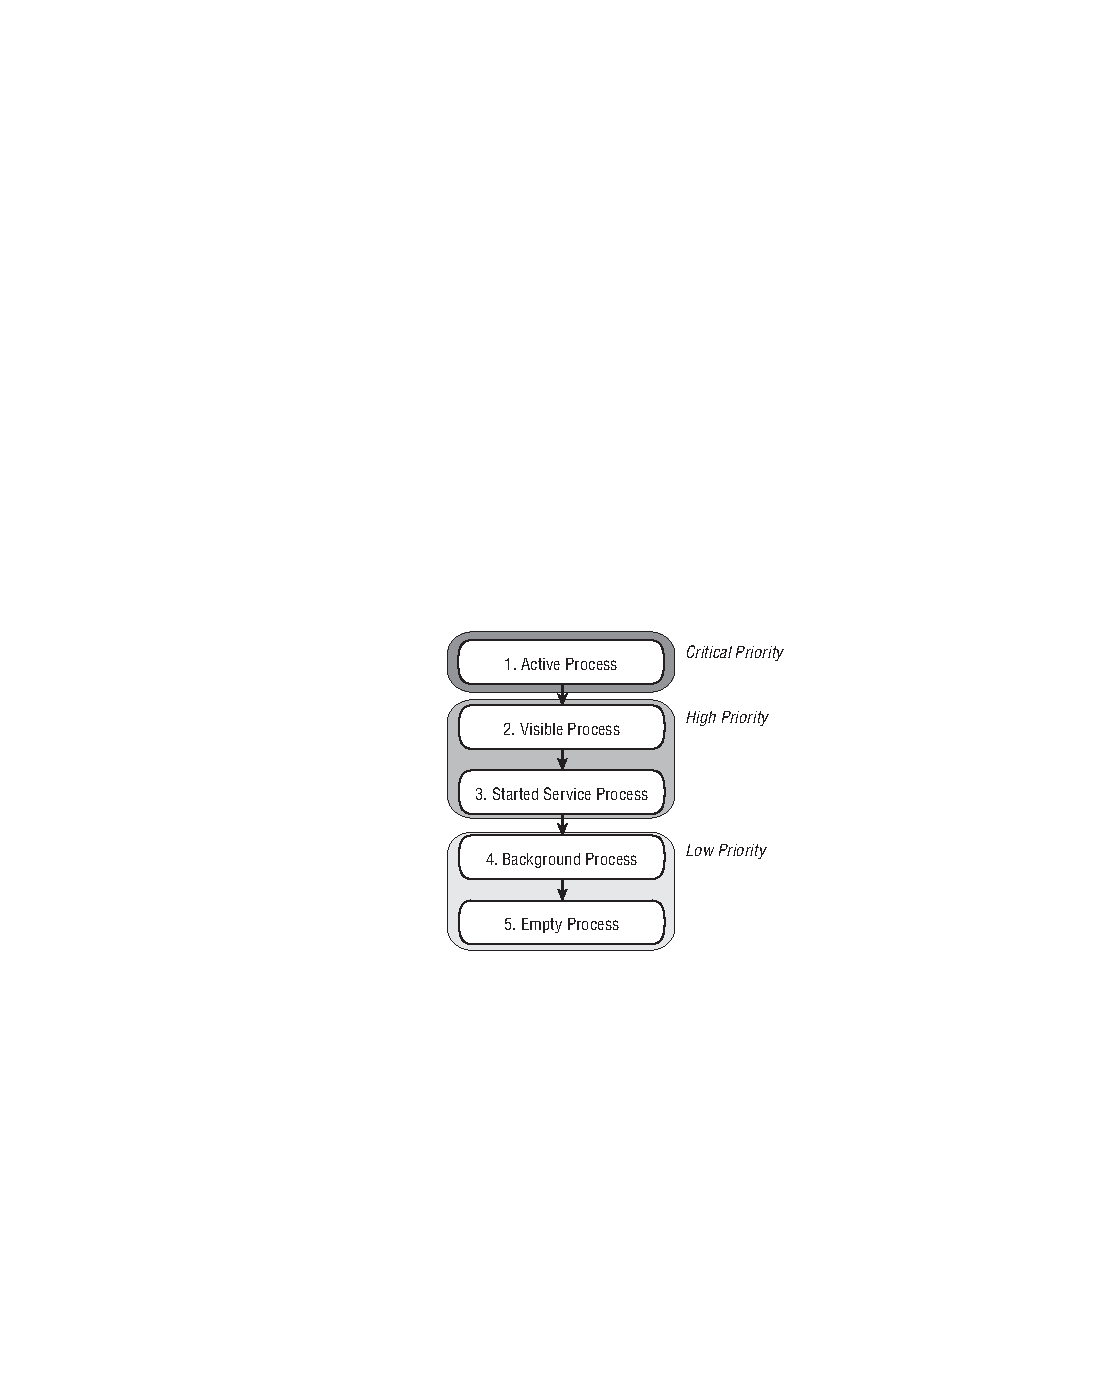
\includegraphics[height=60mm]{figs/PAAD-p51}
    \end{center}

\column{100mm}

  \begin{itemize}
  \item \alert{Prioridad Crítica:}
    \begin{itemize}
      \item \textbf{Procesos activos}: Los que están interactuando con
        el usuario). Hay muy pocos y se les mata sólo como último
        recurso.
    \end{itemize}
  \item \alert{Prioridad Alta:}
    \begin{itemize}
      \item \textbf{Procesos visibles}: Visibles, pero no activos
        (p.ej, parcialmente tapados por otra actividad).  Hay muy
        pocos y se les mata sólo en circunstancias extremas.
      \item \textbf{Procesos de servicios arrancados}: Procesamiento
        que debe continuar aunque no tenga interfaz visible. Se les
        mata sólo en circunstancias extremas.
    \end{itemize}
  \item \alert{Prioridad Baja:}
    \begin{itemize}
      \item \textbf{Procesos de fondo}: Alojan actividades que no caen
        en las categorías anteriores. Hay muchos. Se les mata cuando
        se necesitan recursos para el resto de procesos.
      \item \textbf{Procesos vacíos}: Android mantiene en memoria las
        aplicaciones que han terminado, por si son relanzadas. Se les
        mata rutinariamente.
    \end{itemize}
  \end{itemize}
\end{columns}


\end{frame}



%%%%%%%%%%%%%%%%%%%%%%%%%%%%%%%%%%%%%%%%%%%%
\begin{frame}
\frametitle{Estados de una Actividad (I)}

\begin{center}
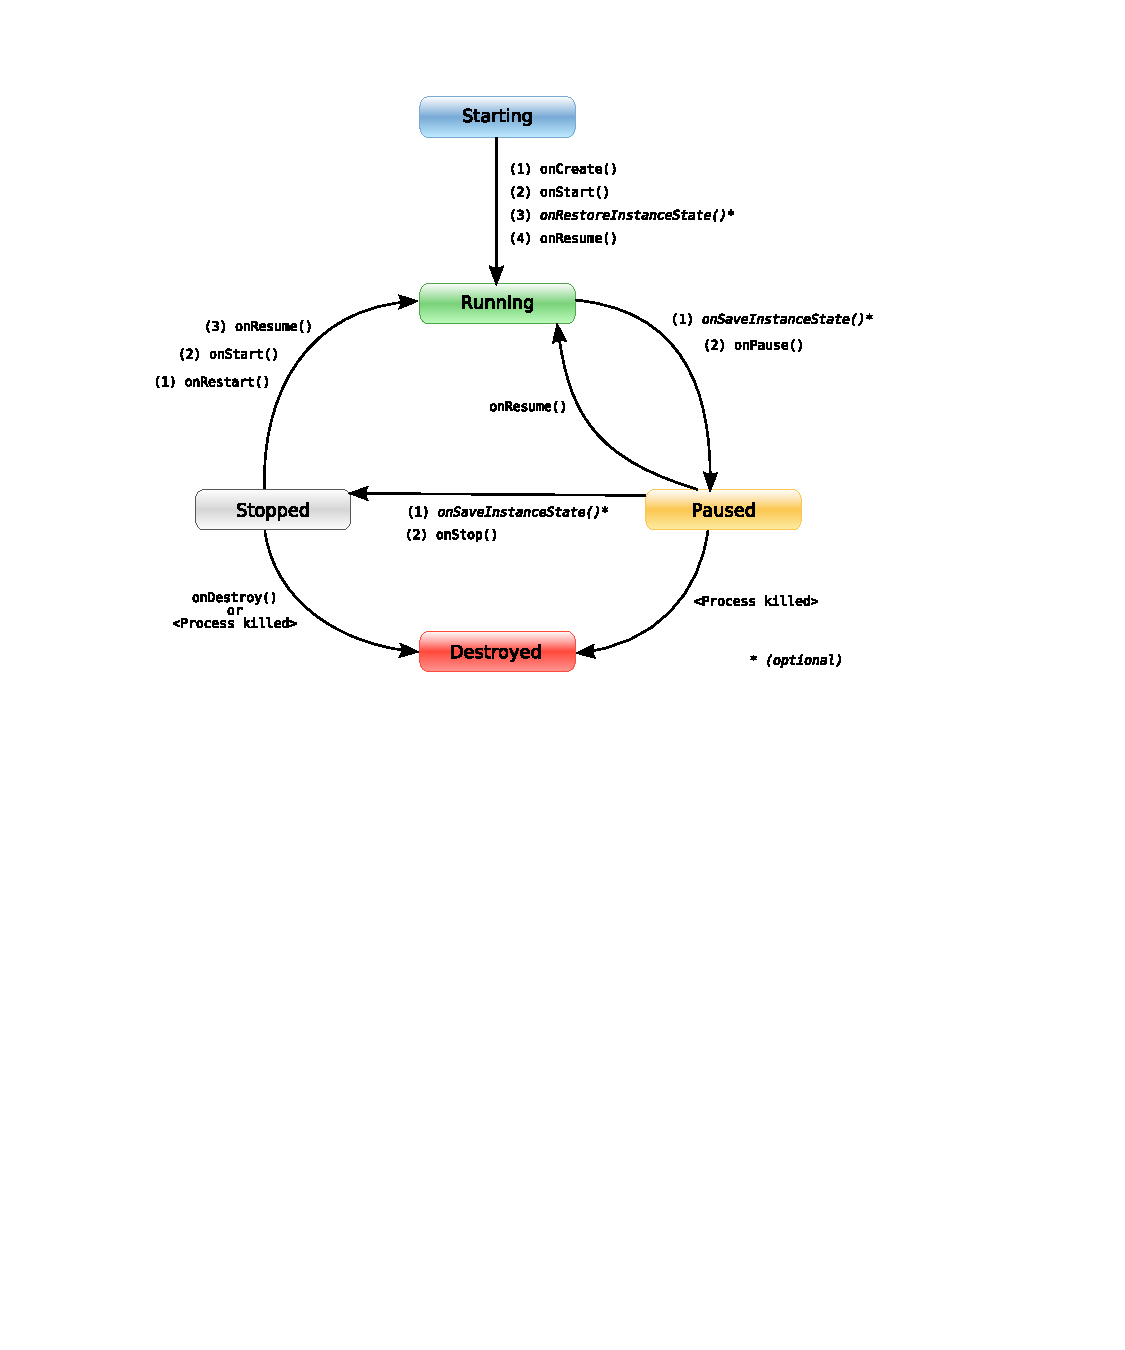
\includegraphics[height=70mm]{figs/PBHA-p37.pdf}  
\end{center}

\end{frame}



%%%%%%%%%%%%%%%%%%%%%%%%%%%%%%%%%%%%%%%%%%%%
\begin{frame}
\frametitle{Estados de una Actividad (II)}

\begin{itemize}
\item \alert{Activo \emph{(Running)}}: La Actividad está encima de la
  pila, es visible, tiene el foco (recibe la entrada del
  usuario). Cuando otra Actividad pase a estar activa, ésta pasará a
  estar pausada.
\item \alert{Pausado \emph{(Paused)}}: La Actividad es visible pero no
  tiene el foco. Se alcanza este estado cuando pasa a activa otra
  Actividad transparente o que no ocupa toda la pantalla. Cuando una
  Actividad es tapada por completo pasa a estar parada.
\item \alert{Parado \emph{(Stopped)}}: Cuando la Actividad no es
  visible. Permanece en memoria reteniendo su estado. Cuando una
  actividad entra en parada puede ser bueno que salve todos sus datos y
  el estado de la Interfaz de usuario.
\item \alert{Destruido \emph{(Destroyed)}}: Cuando la Actividad
    termina, o es matada por el \emph{runtime} de Android. Sale
    de la Pila de Actividades. Necesita ser reiniciada para volver a
    estar activa.
\end{itemize}


\end{frame}



%%%%%%%%%%%%%%%%%%%%%%%%%%%%%%%%%%%%%%%%%%%%
\begin{frame}[fragile]
\frametitle{Estados de una Actividad (III)}

\begin{itemize}
\item En la clase \verb|Activity| existen métodos para ser redefinidos
  \emph{(overrided)} en sus clases derivadas para incluir el código a
  ejecutar en las transiciones entre estados:
  \verb|OnCreate, onStart, onPause, onStop|\ldots.
\item Los métodos redefinidos siempre deben llamar al método de la
  superclase:
\end{itemize}

\begin{tiny}
\begin{block}{}
\begin{java}
// Called at the start of the visible lifetime.
@Override
public void onStart(){
  super.onStart();
  // Apply any required UI change now that the Activity is visible.
}    
\end{java}
\end{block}
\end{tiny}

\end{frame}



%%%%%%%%%%%%%%%%%%%%%%%%%%%%%%%%%%%%%%%%%%%%
\begin{frame}[fragile]
\frametitle{Métodos de transición entre estados (I)}

\begin{itemize}
\item \Verb|\alert{onCreate(Bundle)}|:
  \begin{itemize}
  \item Se invoca cuando la Actividad se arranca por primera vez.
  \item Se utiliza para tareas de inicialización a realizar una sola
    vez, como crear la interfaz de usuario de la Actividad.
  \item Su parámetro es \verb|null| o información de estado guardada
    previamente por \verb|onSaveInstanceState()|.
  \end{itemize}
 
\item \Verb|\alert{onStart()}|:
  \begin{itemize}
  \item Se invoca cuando la Actividad va a ser mostrada al usuario.
  \end{itemize}

\item \Verb|\alert{onResume()}|:
  \begin{itemize}
  \item Se invoca cuando la Actividad va a empezar a interactuar con
    el usuario.
  \end{itemize}

\end{itemize}
\end{frame}


%%%%%%%%%%%%%%%%%%%%%%%%%%%%%%%%%%%%%%%%%%%%
\begin{frame}[fragile]
\frametitle{Métodos de transición entre estados (II)}

\begin{itemize}
\item \Verb|\alert{onPause()}|:
  \begin{itemize}
  \item Se invoca cuando la actividad va a pasar al fondo porque otra
    actividad ha sido lanzada para ponerse delante.
  \item Se utiliza para guardar el estado persistente de la Actividad
  \end{itemize}

\item \Verb|\alert{onStop()}|:
  \begin{itemize}
  \item Se invoca cuando la actividad va a dejar de ser visible y no
    se necesitará durante un tiempo.
  \item Si hay escasez de recursos en el sistema, este método podría
    no llegar a ser invocado y la Actividad ser destruida
    directamente. 
  \end{itemize}

\item \Verb|\alert{onRestart()}|:
  \begin{itemize}
  \item Se invoca cuando la Actividad va a salir del estado de parada
    para volver a estar activa.
  \end{itemize}
\item \Verb|\alert{onDestroy()}|:
  \begin{itemize}
  \item Se invoca cuando la Actividad va a ser destruida.
  \item Si hay escasez de recursos en el sistema, este método podría
    no llegar a ser invocado y la Actividad ser destruida
    directamente. 
  \end{itemize}

\end{itemize}
\end{frame}


%%%%%%%%%%%%%%%%%%%%%%%%%%%%%%%%%%%%%%%%%%%%
\begin{frame}[fragile]
\frametitle{Métodos de transición entre estados (III)}

\begin{itemize}
\item \Verb|\alert{onSaveInstanceState(Bundle)}|:
  \begin{itemize}
  \item Se invoca para permitir a la actividad guardar su estado,
    p.ej: la posición del cursor en una caja de texto.
  \item Normalmente no necesita ser redefinido porque la
    implementación de la clase \verb|Activity| ya guarda todo el
    estado de todos los componentes de la Interfaz de Usuario.
  \end{itemize}
\item \Verb|\alert{onRestoreInstanceState(Bundle)}|: 
  \begin{itemize}
  \item Se invoca para recuperar el estado guardado por
    \verb|onSaveInstanceState()|.
  \item Normalmente no necesita ser redefinido porque la
    implementación de la clase \verb|Activity| ya recupera todo el
    estado de todos los componentes de la Interfaz de Usuario.
  \end{itemize}
\end{itemize}

\end{frame}






%%%%%%%%%%%%%%%%%%%%%%%%%%%%%%%%%%%%%%%%%%%%%%%%%%%%%%%%%%%%%%%%%%%
\section{Recursos de las Aplicaciones Android}
%%%%%%%%%%%%%%%%%%%%%%%%%%%%%%%%%%%%%%%%%%%%%%%%%%%%%%%%%%%%%%%%%%%




%%%%%%%%%%%%%%%%%%%%%%%%%%%%%%%%%%%%%%%%%%%%
\begin{frame}[fragile]
\frametitle{Tipos de recursos}


\begin{itemize}
\item Hay distintos \alert{tipos de recursos}, que se definen en ficheros XML
  alojados en una cierta subcarpeta de \verb|res|:
  \begin{itemize}
  \item Valores simples (carpeta \verb|values|): Strings, colores y
    dimensiones.
  \item Recursos dibujables (carpeta \verb|drawable|): ficheros con
    imágenes, incluyendo el icono de la aplicación
  \item Animaciones (carpeta \verb|anim|)
  \item Menús (carpeta \verb|menu|)
  \item Diseños (carpeta \verb|layout|)
  \item Estilos (carpeta \verb|values|)
  \item Varios (carpeta \verb|xml|)
  \end{itemize}
\end{itemize}
\end{frame}


%%%%%%%%%%%%%%%%%%%%%%%%%%%%%%%%%%%%%%%%%%%%
\begin{frame}[fragile,shrink=10]
\frametitle{Valores simples}

\begin{itemize}

\item Definen Strings, colores o dimensiones
\item Se definen como un elemento:
\begin{tiny}
\begin{block}{}
\begin{xml}
<color name="opaque_red">#f00</color>
\end{xml}
\end{block}
\end{tiny}

\item Las dimensiones pueden tener distintas unidades:
  \verb|px, in, mm, pt, dp, sp|
  \begin{itemize}
  \item \verb|dp|: \emph{Density-independent pixels} (también
    \verb|dip|), pixels independientes de los dpi (puntos por pulgada)
    del dispositivo. Son un valor relativo a un dispositivo de
    160dpi.
  \item \verb|sp|: \emph{Scale-independent pixels}, igual que los
    \verb|dp|, pero también escalados al tamaño de \emph{font} elegido
    por el usuario.
\end{itemize}
\begin{tiny}
\begin{block}{}
\begin{xml}
<dimen name="sixteen_sp">16sp</dimen>
\end{xml}
\end{block}
\end{tiny}

\item Un fichero XML contiene la definición de uno o más de estos elementos.
\item \alert{Todos estos recursos se identifican con el valor de su
    atributo} \Verb|\alert{name}|.
\end{itemize}

\end{frame}


%%%%%%%%%%%%%%%%%%%%%%%%%%%%%%%%%%%%%%%%%%%%%%%%%%%%%%%%
\begin{frame}[fragile]
\frametitle{\emph{Drawables}}

\begin{itemize}
\item Para ficheros de \emph{bitmaps} o de imágenes ``estirables''
  (\verb|.9.png|)
\item También puede definirse uno de estos recursos como un recuadro
  de color: 
\begin{tiny}
\begin{block}{}
\begin{xml}
<drawable name="solid_blue">#0000ff</drawable>
\end{xml}
\end{block}
\end{tiny}
(un fichero XML puede contener uno o más recuadros de color)

\item \alert{Los ficheros se identifican con su nombre de fichero, y
    los recuadros de color con el valor de su atributo} \Verb|\alert{name}|.
\end{itemize}

\end{frame}


%%%%%%%%%%%%%%%%%%%%%%%%%%%%%%%%%%%%%%%%%%%%%%%%%%%%%%%%
\begin{frame}[fragile]
\frametitle{Animaciones}

\begin{itemize}
\item Para realizar animaciones sencillas sobre uno o varios gráficos:
  rotaciones, \emph{fading}, movimiento y estiramiento.
\item Cada animación se define en un fichero XML
\item \alert{Estos recursos se identifican con su nombre de fichero}.
\end{itemize}

\end{frame}


%%%%%%%%%%%%%%%%%%%%%%%%%%%%%%%%%%%%%%%%%%%%%%%%%%%%%%%%
\begin{frame}[fragile]
\frametitle{Menús}

\begin{itemize}
\item Existen tres tipos de menús: Menú de opciones, menú contextual y
  submenú
\item Un menú de opciones o contextual se define en un fichero XML.
\item Un submenú se define dentro de otro menú.
\item \alert{Un menú de opciones o contextual se identifica con su
    nombre de fichero}.
\item \alert{Un submenú se identifica con el valor de su atributo}
  \Verb|\alert{id}|.
\item \alert{Un elemento de un menú también puede ser identificado con el
    valor de su atributo} \Verb|\alert{id}|.
\end{itemize}

\end{frame}


%%%%%%%%%%%%%%%%%%%%%%%%%%%%%%%%%%%%%%%%%%%%%%%%%%%%%%%%
\begin{frame}[fragile]
\frametitle{\emph{Layouts}}

\begin{itemize}
\item Un \emph{layout} se define en un fichero XML.
\item Dentro de un \emph{layout} se definen los elementos que lo
  componen: \emph{Views}, \emph{ViewGroups}
\item \alert{Un \emph{layout} se identifica con su
    nombre de fichero}.
\item \alert{Un elemento de un \emph{layout} también puede ser
    identificado con el valor de su atributo} \Verb|\alert{id}|.
\end{itemize}

\end{frame}


%%%%%%%%%%%%%%%%%%%%%%%%%%%%%%%%%%%%%%%%%%%%%%%%%%%%%%%%
\begin{frame}[fragile]
\frametitle{Estilos}

\begin{itemize}
\item Un estilo es uno o más atributos que se aplican a un elemento.
\item Un tema es uno o más atributos que se aplican a todo lo que hay
  en pantalla. Un tema se asigna como atributo a una Actividad en su
  Manifiesto.
\item Se definen dentro en un elemento \verb|<style>| que contiene
  strings, colores, o referencias a otros recursos.
\item \alert{Un estilo entero se referencia con el
    valor de su atributo} \Verb|\alert{name}|.
\item \alert{Un elemento dentro de un estilo también puede ser
    referenciado de la manera adecuada según el tipo de recurso}.
\end{itemize}

\end{frame}





%%%%%%%%%%%%%%%%%%%%%%%%%%%%%%%%%%%%%%%%%%%%
\begin{frame}[fragile]
\frametitle{Recursos para diferentes idiomas y diferente hardware}

\begin{itemize}
\item Pueden especificarse recursos alternativos para diferentes
  idiomas o diferente hardware con subcarpetas con el mismo nombre que
  la original más un sufijo o conjunto de sufijos.
\item Ejemplos: 
  \begin{itemize}
  \item Valores simples para idioma español: \verb|values-es|
  \item \emph{Layouts} para terminal girado: \verb|layout-land|
  \item \emph{Layouts} para teclado sobreimpresionado:
    \verb|layout-keysexposed|
  \end{itemize}
\item Pueden ponerse varios sufijos encadenados
\item Dentro de esas subcarpetas se colocarán ficheros especializados
  con el mismo nombre que el que tienen en la carpeta básica (ej:
  \verb|strings.xml|)
\item La aplicación al usar un recurso elegirá de entre los
  disponibles aquel en el encajen más sufijos.
\end{itemize}


\end{frame}



%%%%%%%%%%%%%%%%%%%%%%%%%%%%%%%%%%%%%%%%%%%%
\begin{frame}[fragile,shrink=10]
\frametitle{Cambios de configuración en tiempo de ejecución}

\begin{itemize}
\item Una aplicación puede responder a ciertos cambios de configuración
  mientras se ejecuta. 
\item Si lo hace, debe especificarse en el Manifiesto de la
  aplicación:

\begin{tiny}
\begin{block}{}
\begin{xml}
<activity android:name=".TodoList"
          android:label="@string/app_name"
          android:theme="@style/TodoTheme"
          android:configChanges="orientation|keyboardHidden"/>
\end{xml}
\end{block}
\end{tiny}

\item Cuando se produzca el cambio se invocará el método
  \verb|onConfigurationChanged| en la Actividad:

\begin{tiny}
\begin{block}{}
\begin{java}
@Override
public void onConfigurationChanged(Configuration _newConfig) {
  super.onConfigurationChanged(_newConfig);
  [ ... Update any UI based on resource values ... ]
  if (_newConfig.orientation == Configuration.ORIENTATION_LANDSCAPE) {
    [ ... React to different orientation ... ]
  }
  if (_newConfig.keyboardHidden == Configuration.KEYBOARDHIDDEN_NO) {
    [ ... React to changed keyboard visibility ... ]
  }
}
\end{java}
\end{block}
\end{tiny}


\end{itemize}

\end{frame}



%%%%%%%%%%%%%%%%%%%%%%%%%%%%%%%%%%%%%%%%%%%%
\begin{frame}[fragile,shrink=15]
\frametitle{Utilización de recursos en el código (I)}

\begin{itemize}
\item Se accede a los recursos de una aplicación a través de la clase
  estática \Verb|\alert{R}|, regenerada a partir de los ficheros XML cada vez
  que se recompila el proyecto.
\item La clase \verb|R| incluye subclases estáticas para cada uno de
  los tipos de recursos para los que se ha definido al menos un
  recurso. Ej: \Verb|\alert{R.string}|, \Verb|\alert{R.drawable}|
\item Cada subclase expone sus recursos asociados como variables, con
  nombre igual a los identificadores de los recursos. Ej:
  \Verb|\alert{R.string.app_name}|, \Verb|\alert{R.drawable.icon}|
\item El valor de estas variables es una referencia al recurso, no una
  instancia del recurso.
\vspace{2mm}
\item Cuando un constructor o un método (como \verb|setContentView|)
  acepta como parámetro un identificador de recurso, se le puede pasar
  una de estas variables:
\begin{scriptsize}
\begin{block}{}
\begin{java}
// Inflate a layout resource.
setContentView(R.layout.main);
// Display a transient dialog box that displays the
// error message string resource.
Toast.makeText(this, R.string.app_error, Toast.LENGTH_LONG).show();
\end{java}
\end{block}
\end{scriptsize}
\end{itemize}

\end{frame}



%%%%%%%%%%%%%%%%%%%%%%%%%%%%%%%%%%%%%%%%%%%%
\begin{frame}[fragile]
\frametitle{Utilización de recursos en el código (II)}

\begin{itemize}
\item La tabla de recursos de una aplicación está representada por una
  instancia de la clase \Verb|\alert{Resources}|.
\item Cuando se necesita una instancia del recurso se usan métodos
  \emph{helper} para extraerlos de la tabla de recursos.
\item La clase \verb|Resources| incluye \emph{getters} para cada tipo
  de recursos disponible, a los que se pasa la variable (referencia)
  del recurso del que se quiere una instancia:
\begin{tiny}
\begin{block}{}
\begin{java}
Resources myResources = getResources();
CharSequence styledText = myResources.getText(R.string.stop_message);
Drawable icon = myResources.getDrawable(R.drawable.app_icon);

int opaqueBlue = myResources.getColor(R.color.opaque_blue);

float borderWidth = myResources.getDimension(R.dimen.standard_border);

Animation tranOut;
tranOut = AnimationUtils.loadAnimation(this, R.anim.spin_shrink_fade);

String[] stringArray;
stringArray = myResources.getStringArray(R.array.string_array);

int[] intArray = myResources.getIntArray(R.array.integer_array);
\end{java}
\end{block}
\end{tiny}



\end{itemize}

\end{frame}



%%%%%%%%%%%%%%%%%%%%%%%%%%%%%%%%%%%%%%%%%%%%
\begin{frame}[fragile,shrink=5]
\frametitle{Referenciación de Recursos en otros Recursos}

\begin{itemize}
\item Para referenciar un recurso en otro recurso se utiliza la
  notación \Verb|\alert{@}|:
\begin{tiny}
\begin{block}{}
\begin{xml}
atributo="@[nombre_paquete:]tipo_recurso/id_recurso"
\end{xml}
\end{block}
\end{tiny}
(el nombre de paquete puede omitirse si es del mismo paquete)

\item Ejemplo:

\begin{tiny}
\begin{block}{}
\begin{xml}
<?xml version="1.0" encoding="utf-8"?>
<LinearLayout
  xmlns:android="http://schemas.android.com/apk/res/android"
  android:orientation="vertical"
  android:layout_width="fill_parent"
  android:layout_height="fill_parent"
  android:padding="@dimen/standard_border">
  <EditText
     android:id="@+id/myEditText"
     android:layout_width="fill_parent"
     android:layout_height="wrap_content"
     android:text="@string/stop_message"
     android:textColor="@color/opaque_blue"
  />
</LinearLayout>
\end{xml}
\end{block}
\end{tiny}


\end{itemize}



\end{frame}



%%%%%%%%%%%%%%%%%%%%%%%%%%%%%%%%%%%%%%%%%%%%
\begin{frame}[fragile,shrink=10]
\frametitle{Referenciación de Recursos del Sistema}

\begin{itemize}
\item Las aplicaciones nativas de Android externalizan muchos de sus
  recursos para que sean accesibles desde otras aplicaciones.
\item Para acceder a ellos en el código Java se utiliza
  \Verb|\alert{android.R}| en vez de \verb|R|:
\begin{tiny}
\begin{block}{}
\begin{java}
CharSequence httpError = getString(android.R.string.httpErrorBadUrl);
\end{java}
\end{block}
\end{tiny}

\item Para acceder desde otros recursos, se utiliza
  \Verb|\alert{android}| como nombre de paquete:
\begin{tiny}
\begin{block}{}
\begin{xml}
<EditText
   android:id="@+id/myEditText"
   android:layout_width="fill_parent"
   android:layout_height="wrap_content"
   android:text="@android:string/httpErrorBadUrl"
   android:textColor="@android:color/darker_gray"
/>
\end{xml}
\end{block}
\end{tiny}

\item También es posible acceder a recursos del tema actual (para
  mantener consistencia con el resto de aplicaciones), con
  \Verb|\alert{?}|:
\begin{tiny}
\begin{block}{}
\begin{xml}
   android:textColor=?android:textColor"
\end{xml}
\end{block}
\end{tiny}

\end{itemize}

\end{frame}


%%%%%%%%%%%%%%%%%%%%%%%%%%%%%%%%%%%%%%%%%%%%%%%%%%%%%%%%%%%%%%%%%%%
\section{Creación de Interfaces de Usuario: \texttt{Views}}
%%%%%%%%%%%%%%%%%%%%%%%%%%%%%%%%%%%%%%%%%%%%%%%%%%%%%%%%%%%%%%%%%%%

% vistas
% layouts
% controles compuestos
% controles definidos por el usuario
% menús


%%%%%%%%%%%%%%%%%%%%%%%%%%%%%%%%%%%%%%%%%%%%
\begin{frame}[fragile]
\frametitle{Terminología}

\begin{itemize}
\item \alert{Vistas \emph{(Views)}}: Clase básica que representa a un
  elemento básico de IU en Android. En otros tipo de aplicaciones
  se utiliza el nombre de controles o \emph{widgets}.
\item Todos los componentes visuales en Android descienden de la clase
  \verb|View|.
\item \alert{Grupos de Vistas \emph{(ViewGroups)}}: Extensiones de la
  clase \verb|View| para crear controles compuestos que contienen
  múltiples \emph{Views} hijas.
\item \alert{Diseños \emph{(Layouts)}}: Extensiones de la clase
  \verb|ViewGroup| para gestionar la disposición de sus \emph{Views}
  hijas.
\end{itemize}

\end{frame}



%%%%%%%%%%%%%%%%%%%%%%%%%%%%%%%%%%%%%%%%%%%%
\begin{frame}[fragile]
\frametitle{Creación de la IU de una Actividad con \emph{Views}}

\begin{itemize}
\item La forma habitual es establecer el \emph{Layout} al principio
  del método \verb|onCreate|.
\item Una vez establecido, pueden obtenerse referencias a las
  \emph{Views} contenidas en el \emph{Layout} llamando al método
  \Verb|\alert{findViewById}|:

\begin{tiny}
\begin{block}{}
\begin{java}
@Override
public void onCreate(Bundle savedInstanceState) {
  super.onCreate(savedInstanceState);

  setContentView(R.layout.main);

  TextView myTextView = (TextView)findViewById(R.id.myTextView);
\end{java}
\end{block}
\end{tiny}

\end{itemize}


\end{frame}



%%%%%%%%%%%%%%%%%%%%%%%%%%%%%%%%%%%%%%%%%%%%
\begin{frame}[fragile]
\frametitle{\emph{Views} estándar habituales}

\begin{itemize}
\item \Verb|\alert{TextView}|: Etiqueta de texto de solo lectura.
\item \Verb|\alert{EditText}|: Caja de texto editable, que acepta
  entradas multilínea.
\item \Verb|\alert{ListView}|: \emph{ViewGroup} que gestiona un grupo
  de \emph{Views} para mostrarlo en forma de lista, usando por
  defecto un \emph{TextView} para cada elemento.
\item \Verb|\alert{Spinner}|: Control compuesto que muestra un
  \emph{TextView} con una \emph{ListView} asociada para elegir uno de
  sus elementos para ser mostrado en el \emph{TextView}.
\item \Verb|\alert{Button}|: Botón pulsable estándar.
\item \Verb|\alert{Checkbox}|: Botón de dos estados representado por
  un caja marcada o desmarcada.
\item \Verb|\alert{RadioButton}|: Varios botones de dos estados, agrupados de
  forma que sólo uno del grupo puede estar activado.
\end{itemize}

\end{frame}

%%%%%%%%%%%%%%%%%%%%%%%%%%%%%%%%%%%%%%%%%%%%%%%%%%%%%%%%%%%%%%%%%%%
\section{Creación de Interfaces de Usuario: \texttt{Layouts}}
%%%%%%%%%%%%%%%%%%%%%%%%%%%%%%%%%%%%%%%%%%%%%%%%%%%%%%%%%%%%%%%%%%%


%%%%%%%%%%%%%%%%%%%%%%%%%%%%%%%%%%%%%%%%%%%%
\begin{frame}[fragile]
\frametitle{\emph{Layouts} estándar habituales}

\begin{itemize}
\item \Verb|\alert{FrameLayout}|: Coloca cada \emph{View} en la
  esquina izquierda. Cada nueva \emph{View} que se añade tapa a la anterior.
\item \Verb|\alert{LinearLayout}|: Coloca cada \emph{View} hija en
  línea, de forma horizontal (una fila de \emph{Views}) o vertical
  (una columna de \emph{Views}).
\item \Verb|\alert{TableLayout}|: Coloca las \emph{Views} en forma de
  tabla
\item \Verb|\alert{RelativeLayout}|: Las posiciones de cada \emph{View}
  hija es relativa a las otras y a los bordes de la pantalla
\item \Verb|\alert{AbsoluteLayout}|: Las posiciones de cada \emph{View}
  hija se define en coordenadas absolutas
\end{itemize}

\end{frame}



%%%%%%%%%%%%%%%%%%%%%%%%%%%%%%%%%%%%%%%%%%%%
\begin{frame}[fragile]
\frametitle{Ejemplo:}

\begin{tiny}
\begin{block}{}
\begin{xml}
<?xml version="1.0" encoding="utf-8"?>
<LinearLayout xmlns:android="http://schemas.android.com/apk/res/android"
  android:orientation="vertical"
  android:layout_width="fill_parent"
  android:layout_height="fill_parent">
  <TextView
     android:layout_width="fill_parent"
     android:layout_height="wrap_content"
     android:text="Enter Text Below"
  />
  <EditText
     android:layout_width="fill_parent"
     android:layout_height="wrap_content"
     android:text="Text Goes Here!"
  />
</LinearLayout>
\end{xml}
\end{block}
\end{tiny}


\end{frame}



%%%%%%%%%%%%%%%%%%%%%%%%%%%%%%%%%%%%%%%%%%%%%%%%%%%%%%%%%%%%%%%%%%%
\section{Creación de Interfaces de Usuario: Creación de nuevas \texttt{Views}}
%%%%%%%%%%%%%%%%%%%%%%%%%%%%%%%%%%%%%%%%%%%%%%%%%%%%%%%%%%%%%%%%%%%

%%%%%%%%%%%%%%%%%%%%%%%%%%%%%%%%%%%%%%%%%%%%
\begin{frame}[fragile,shrink=25]
\frametitle{Creación de nuevas \emph{Views} a partir de las existentes}

\begin{itemize}
\item Se extiende una \emph{View} ya existente, redefiniendo los
  métodos que definen su apariencia y su comportamiento:
\end{itemize}

\begin{tiny}
\begin{block}{MyTextView.java}
\begin{java}
public class MyTextView extends TextView {
  public MyTextView (Context context, AttributeSet ats, int defStyle) {
    super(context, ats, defStyle);
  }

  public MyTextView (Context context) {
    super(context);
  }

  public MyTextView (Context context, AttributeSet attrs) {
    super(context, attrs);
  }

  @Override
  public void onDraw(Canvas canvas) {
    [ ... Draw things on the canvas under the text ... ]

    // Render the text as usual using the TextView base class.
    super.onDraw(canvas);

    [ ... Draw things on the canvas over the text ... ]
  }

  @Override
  public boolean onKeyDown(int keyCode, KeyEvent keyEvent) {
    [ ... Perform some special processing ... ]
    [ ... based on a particular key press ... ]

    // Use the existing functionality implemented by
    // the base class to respond to a key press event.
    return super.onKeyDown(keyCode, keyEvent);
  }
}
\end{java}
\end{block}
\end{tiny}

\end{frame}



%%%%%%%%%%%%%%%%%%%%%%%%%%%%%%%%%%%%%%%%%%%%
\begin{frame}[fragile,shrink=10]
\frametitle{Mejora del aspecto de la \emph{TodoList} (I)}

\begin{itemize}
\item Creamos una nueva \verb|TodoListItemView| extendiendo \verb|TextView|:
\end{itemize}

\begin{tiny}
\begin{block}{src/com.clau.todolist/TodoListItemView.java}
\begin{java}
package com.clau.todolist;
import android.content.Context;
import android.content.res.Resources;
import android.graphics.Canvas;
import android.graphics.Paint;
import android.util.AttributeSet;
import android.widget.TextView;

public class TodoListItemView extends TextView {
  public TodoListItemView (Context context, AttributeSet ats, int ds) {
    super(context, ats, ds);
    init();
  }

  public TodoListItemView (Context context) {
    super(context);
    init();
  }

  public TodoListItemView (Context context, AttributeSet attrs) {
    super(context, attrs);
    init();
  }
  private void init() {
  }

  @Override
  public void onDraw(Canvas canvas) {
    // Use the base TextView to render the text.
    super.onDraw(canvas);
  }
}
\end{java}
\end{block}
\end{tiny}


\end{frame}


%%%%%%%%%%%%%%%%%%%%%%%%%%%%%%%%%%%%%%%%%%%%
\begin{frame}[fragile]
\frametitle{Mejora del aspecto de la \emph{TodoList} (II)}

\begin{itemize}
\item Creamos un nuevo \verb|colors.xml| en \verb|res/values|:
\begin{tiny}
\begin{block}{res/values/colors.xml}
\begin{xml}
<?xml version="1.0" encoding="utf-8"?>
<resources>
  <color name="notepad_paper">#AAFFFF99</color>
  <color name="notepad_lines">#FF0000FF</color>
  <color name="notepad_margin">#90FF0000</color>
  <color name="notepad_text">#AA0000FF</color>
</resources>
\end{xml}
\end{block}
\end{tiny}

\item Creamos un nuevo \verb|dimens.xml| en \verb|res/values|:
\begin{tiny}
\begin{block}{res/values/dimens.xml}
\begin{xml}
<?xml version="1.0" encoding="utf-8"?>
<resources>
  <dimen name="notepad_margin">30px</dimen>
</resources>
\end{xml}
\end{block}
\end{tiny}


\end{itemize}


\end{frame}

%%%%%%%%%%%%%%%%%%%%%%%%%%%%%%%%%%%%%%%%%%%%
\begin{frame}[fragile]
\frametitle{Mejora del aspecto de la \emph{TodoList} (III)}

\begin{itemize}
\item Ahora podemos incluir el método \verb|init| en
  \verb|TodoListItemView|:
\end{itemize}

\begin{tiny}
\begin{block}{src/com.clau.todolist/TodoListItemView.java (fragmento)}
\begin{java}
private Paint marginPaint;
private Paint linePaint;
private int paperColor;
private float margin;

private void init() {
  // Get a reference to our resource table.
  Resources myResources = getResources();

  // Create the paint brushes we will use in the onDraw method.
  marginPaint = new Paint(Paint.ANTI_ALIAS_FLAG);
  marginPaint.setColor(myResources.getColor(R.color.notepad_margin));
  linePaint = new Paint(Paint.ANTI_ALIAS_FLAG);
  linePaint.setColor(myResources.getColor(R.color.notepad_lines));

  // Get the paper background color and the margin width.
  paperColor = myResources.getColor(R.color.notepad_paper);
  margin = myResources.getDimension(R.dimen.notepad_margin);
}
\end{java}
\end{block}
\end{tiny}


\end{frame}


%%%%%%%%%%%%%%%%%%%%%%%%%%%%%%%%%%%%%%%%%%%%
\begin{frame}[fragile]
\frametitle{Mejora del aspecto de la \emph{TodoList} (IV)}

\begin{itemize}
\item Refinamos el método \verb|onDraw| utilizando las variables de
  instancia inicialidadas en \verb|init|:
\end{itemize}

\begin{tiny}
\begin{block}{src/com.clau.todolist/TodoListItemView.java (fragmento)}
\begin{java}
  @Override
  public void onDraw(Canvas canvas) {
    // Color as paper
    canvas.drawColor(paperColor);

    // Draw ruled lines
    canvas.drawLine(0, 0, getMeasuredHeight(), 0, linePaint);
    canvas.drawLine(0, getMeasuredHeight(),
    getMeasuredWidth(), getMeasuredHeight(),
    linePaint);

    // Draw margin
    canvas.drawLine(margin, 0, margin, getMeasuredHeight(), marginPaint);

    // Move the text across from the margin
    canvas.save();
    canvas.translate(margin, 0);
  
    // Use the base TextView to render the text.
    super.onDraw(canvas);
    canvas.restore();
  }
\end{java}
\end{block}
\end{tiny}

\end{frame}



%%%%%%%%%%%%%%%%%%%%%%%%%%%%%%%%%%%%%%%%%%%%
\begin{frame}[fragile]
\frametitle{Mejora del aspecto de la \emph{TodoList} (V)}

\begin{itemize}
\item Creamos un nuevo \emph{Layout} para especificar cómo se
  dispondrán los elementos de la lista usando la nueva \emph{View}:
\end{itemize}

\begin{tiny}
\begin{block}{res/layout/todolist\_item.xml}
\begin{xml}
<?xml version="1.0" encoding="utf-8"?>
<com.clau.todolist.TodoListItemView
   xmlns:android="http://schemas.android.com/apk/res/android"
   android:layout_width="fill_parent"
   android:layout_height="fill_parent"
   android:padding="10dp"
   android:scrollbars="vertical"
   android:textColor="@color/notepad_text"
   android:fadingEdge="vertical"
/>
\end{xml}
\end{block}
\end{tiny}

\end{frame}



%%%%%%%%%%%%%%%%%%%%%%%%%%%%%%%%%%%%%%%%%%%%
\begin{frame}[fragile]
\frametitle{Mejora del aspecto de la \emph{TodoList} (VI)}

\begin{itemize}
\item Ahora en el \verb|onCreate| de \verb|ToDoList.java|
  reemplazamos los parámetros pasados al \verb|ArrayAdapter| para
  hacer uso del nuevo \emph{Layout}.
\item ANTES:
\begin{tiny}
\begin{block}{src/com.clau.todolist/TodoListItemView.java (fragmento)}
\begin{java}
  final ArrayList<String> todoItems = new ArrayList<String>();
  final ArrayAdapter<String> aa;
  aa = new ArrayAdapter<String>(this,
    android.R.layout.simple_list_item_1, todoItems);
  myListView.setAdapter(aa);
\end{java}
\end{block}
\end{tiny}

\item \alert{AHORA}:
\begin{tiny}
\begin{block}{src/com.clau.todolist/TodoListItemView.java (fragmento)}
\begin{java}
  final ArrayList<String> todoItems = new ArrayList<String>();
  int resID = R.layout.todolist_item;
  final ArrayAdapter<String> aa;
  aa = new ArrayAdapter<String>(this, resID, todoItems);
  myListView.setAdapter(aa);
\end{java}
\end{block}
\end{tiny}

\end{itemize}


\end{frame}

%%%%%%%%%%%%%%%%%%%%%%%%%%%%%%%%%%%%%%%%%%%%%%%%%%%%%%%%%%%%%%%%%%%
\section[Creación de IU: Creación de Controles Compuestos]{Creación de Interfaces de Usuario: Creación de Controles Compuestos}
%%%%%%%%%%%%%%%%%%%%%%%%%%%%%%%%%%%%%%%%%%%%%%%%%%%%%%%%%%%%%%%%%%%


%%%%%%%%%%%%%%%%%%%%%%%%%%%%%%%%%%%%%%%%%%%%%%%%%%%%%%%%%%
\begin{frame}[fragile]
\frametitle{Creación de controles compuestos (I)}

\begin{itemize}
\item Un \alert{Control Compuesto} es aquel formado por múltiples
  \emph{Views} que trabajan juntos.
\item Al crearlo se define su disposición, apariencia y la interación
  entre sus \emph{Views}.
\item Se crean extendiendo un \verb|ViewGroup| (o más bien un
  \emph{Layout}):

\begin{tiny}
\begin{block}{MyCompoundView.java}
\begin{java}
public class MyCompoundView extends LinearLayout {
  public MyCompoundView(Context context) {
    super(context);
  }
  public MyCompoundView(Context context, AttributeSet attrs) {
    super(context, attrs);
  }
}
\end{java}
\end{block}
\end{tiny}


\end{itemize}

\end{frame}


%%%%%%%%%%%%%%%%%%%%%%%%%%%%%%%%%%%%%%%%%%%%%%%%%%%%%%%%%%
\begin{frame}[fragile]
\frametitle{Creación de controles compuestos (II)}

\begin{itemize}
\item Para diseñar su interfaz de usuario se utiliza un \emph{Layout}:
\begin{tiny}
\begin{block}{clearable\_edit\_text.xml}
\begin{xml}
<?xml version="1.0" encoding="utf-8"?>
<LinearLayout xmlns:android="http://schemas.android.com/apk/res/android"
  android:orientation="vertical"
  android:layout_width="fill_parent"
  android:layout_height="fill_parent">
  <EditText
     android:id="@+id/editText"
     android:layout_width="fill_parent"
     android:layout_height="wrap_content"
  />
  <Button
     android:id="@+id/clearButton"
     android:layout_width="fill_parent"
     android:layout_height="wrap_content"
     android:text="Clear"
  />
</LinearLayout>
\end{xml}
\end{block}
\end{tiny}

\end{itemize}

\end{frame}


%%%%%%%%%%%%%%%%%%%%%%%%%%%%%%%%%%%%%%%%%%%%%%%%%%%%%%%%%%
\begin{frame}[fragile]
\frametitle{Creación de controles compuestos (III)}

\begin{itemize}
\item Para asignar el \emph{Layout} al nuevo control compuesto hay que
  redefinir su constructor:
\begin{tiny}
\begin{block}{MyCompoundView.java (fragmento)}
\begin{java}
EditText editText;
Button clearButton;

public ClearableEditText(Context context) {
    super(context);
 
   // Inflate the view from the layout resource.
    String infService = Context.LAYOUT_INFLATER_SERVICE;
    LayoutInflater li;
    li = (LayoutInflater)getContext().getSystemService(infService);
    li.inflate(R.layout.clearable_edit_text, this, true);

    // Get references to the child controls.
    editText = (EditText)findViewById(R.id.editText);
    clearButton = (Button)findViewById(R.id.clearButton);

    // Hook up the functionality
    hookupButton();
  }
}
\end{java}
\end{block}
\end{tiny}

\end{itemize}

\end{frame}

%%%%%%%%%%%%%%%%%%%%%%%%%%%%%%%%%%%%%%%%%%%%%%%%%%%%%%%%%%%%%%%%%%%
\section{Creación de Interfaces de Usuario: Menús}
%%%%%%%%%%%%%%%%%%%%%%%%%%%%%%%%%%%%%%%%%%%%%%%%%%%%%%%%%%%%%%%%%%%


%%%%%%%%%%%%%%%%%%%%%%%%%%%%%%%%%%%%%%%%%%%%%%%%%%%%%%%%%%%%%%%
\begin{frame}
\frametitle{Tipos de Menú}



\begin{itemize}
\item \alert{Menú de Opciones}: El que aparece cuando se pulsa el
  botón ``Menú'' o ``M'' del terminal. Consta de un menú de iconos y,
  en su caso, de un menú expandido:
  \begin{itemize}
  \item \textbf{Menú de Iconos}: Hasta 6 elementos con un icono y/o
    texto.  En cada elemento puede ir un submenú. Si se definen más de
    6 elementos, aparece un elemento llamado ``Más'' que mostrará el
    menú expandido.
  \item \textbf{Menú Expandido}: Lista desplazable de los elementos del
    menú de opciones que no entraban dentro del menú de iconos.
  \end{itemize}
\item \alert{Menú Contextual}: Menú que se despliega al pulsar el
  botón central del terminal, o al tocar prolongadamente la pantalla
  táctil.
\item \alert{Submenú}: Menú flotante que se despliega al seleccionar
  una entrada definida como submenú en alguno de los menús
  anteriores. Dentro de un submenú NO puede haber otro.
\end{itemize}

\end{frame}


%%%%%%%%%%%%%%%%%%%%%%%%%%%%%%%%%%%%%%%%%%%%%%%%%%%
\begin{frame}[fragile,shrink=40]
\frametitle{Creación de un Menú de Opciones para una Actividad}

\begin{itemize}
\item Hay que redefinir el método
  \Verb|\alert{OnCreateOptionsMenu}|, que se invocará la primera vez
  que se muestre el menú de opciones de la Actividad.
\item En la implementación redefinida es necesario llamar al método
  de la clase \verb|Activity|.
\item Para añadir entradas al menú se utiliza el método \Verb|\alert{add}|
  de la clase \verb|Menu|, que requiere los siguientes parámetros:
  \begin{itemize}
  \item un identificador de grupo para poder agrupar entradas
  \item un identificador de la entrada, que permitirá saber qué
    entrada se ha pulsado cuando se invoque el manejador
    \verb|onOptionsItemSelected|. Cada identificador de una
    entrada debería declararse como atributo de clase de la
    Actividad.
  \item un número de orden para la colocación de la entrada en el
    menú
  \item el texto de la entrada
  \end{itemize}
\end{itemize}

\begin{scriptsize}
\begin{block}{}
\begin{java}
static final private int MENU_ITEM = Menu.FIRST;

@Override
public boolean onCreateOptionsMenu(Menu menu) {
  super.onCreateOptionsMenu(menu);

  // Group ID
  int groupId = 0;
  // Unique menu item identifier. Used for event handling.
  int menuItemId = MENU_ITEM;
  // The order position of the item
  int menuItemOrder = Menu.NONE;
  // Text to be displayed for this menu item.
  int menuItemText = R.string.menu_item;

  // Create the menu item and keep a reference to it.
  MenuItem menuItem = menu.add(groupId, menuItemId,
                               menuItemOrder, menuItemText);
  return true;
}
\end{java}
\end{block}
\end{scriptsize}


\end{frame}


%%%%%%%%%%%%%%%%%%%%%%%%%%%%%%%%%%%%%%%%%%%%%%%%%%%
\begin{frame}[fragile]
\frametitle{Elementos del Menú de Opciones}

\begin{itemize}
\item La clase \verb|MenuItem| permite añadir detalles adicionales a
  la entrada:
  \begin{itemize}
  \item \emph{Checkboxes} o \emph{Radio Buttons}, sólo visibles en el menú expandido o en un submenú.
  \item Atajos de teclado
  \item Títulos abreviados
  \item Iconos (sólo visibles en el menú de iconos)
  \item Manejador a ejecutar cuando se seleccione este elemento (NO
    recomendado, es más eficiente usar \verb|onOptionsItemSelected|)
  \item Intenciones, que serán activadas cuando se seleccione este
    elemento.
  \end{itemize}
\end{itemize}


\end{frame}


%%%%%%%%%%%%%%%%%%%%%%%%%%%%%%%%%%%%%%%%%%%%%%%%%%%
\begin{frame}[fragile]
\frametitle{Modificación dinámica del Menú de Opciones}

\begin{itemize}
\item Puede modificarse un menú cada vez que se muestra redefiniendo
  el método \Verb|\alert{onPrepareOptionsMenu}|:
\end{itemize}

\begin{scriptsize}
\begin{block}{}
\begin{java}
@Override
public boolean onPrepareOptionsMenu(Menu menu) {
  super.onPrepareOptionsMenu(menu);

  MenuItem menuItem = menu.findItem(MENU_ITEM);

  [ ... modify menu items ... ]

  return true;
}
\end{java}
\end{block}
\end{scriptsize}


\end{frame}


%%%%%%%%%%%%%%%%%%%%%%%%%%%%%%%%%%%%%%%%%%%%%%%%%%%
\begin{frame}[fragile]
\frametitle{Manejar las selecciones del menú}

\begin{itemize}
\item A través del único manejador \Verb|\alert{onOptionsItemSelected}|.
\item El elemento seleccionado se recibe como parámetro \verb|MenuItem|.
\item Habrá que comparar su identificador con los establecidos al
  crear el menú:
\end{itemize}

\begin{tiny}
\begin{block}{}
\begin{java}
public boolean onOptionsItemSelected(MenuItem item) {
  super.onOptionsItemSelected(item);

  // Find which menu item has been selected
  switch (item.getItemId()) {

    // Check for each known menu item
    case (MENU_ITEM):
      [ ... Perform menu handler actions ... ]
      return true;
  }

  // Return false if you have not handled the menu item.
  return false;
}

\end{java}
\end{block}
\end{tiny}

\end{frame}


%%%%%%%%%%%%%%%%%%%%%%%%%%%%%%%%%%%%%%%%%%%%%%%%%%%
\begin{frame}[fragile]
\frametitle{Creación de un Submenú}

\begin{itemize}
\item A través de \Verb|\alert{addSubMenu}|, que admite los mismos
  parámetros que \Verb|add| para añadir elementos normales.
\item Los elementos de dentro del submenú se gestionan igual que los
  del menú de opciones.
\item Adicionalmente se puede añadir un icono para el menú de opciones
  y para la cabecera del submenú cuando se muestre.
\end{itemize}

\begin{tiny}
\begin{block}{}
\begin{java}
  SubMenu sub = menu.addSubMenu(0, 0, Menu.NONE, "Submenu");
  sub.setHeaderIcon(R.drawable.icon);
  sub.setIcon(R.drawable.icon);

  MenuItem submenuItem = sub.add(0, 0, Menu.NONE, "Submenu Item");
\end{java}
\end{block}
\end{tiny}


\end{frame}


%%%%%%%%%%%%%%%%%%%%%%%%%%%%%%%%%%%%%%%%%%%%%%%%%%%
\begin{frame}[fragile, shrink=23]
\frametitle{Menús Contextuales}

\begin{itemize}
% \item Puede crearse un menú contextual asociado a cualquier
%   \verb|View|, redefiniendo su método
%   \Verb|\alert{onCreateContextMenu}|. Esté menú estará disponible para
%   cualquier Actividad que incluya esa \emph{View}.
% \begin{scriptsize}
% \begin{block}{}
% \begin{java}
% @Override
% public void onCreateContextMenu(ContextMenu menu) {
%   super.onCreateContextMenu(menu);
%   menu.add("ContextMenuItem1");
% }
% \end{java}
% \end{block}
% \end{scriptsize}

\item Puede crearse un menú contextual para una Actividad redefiniendo
  su método \Verb|\alert{onCreateContextMenu}| y registrando la
  \emph{View} que lo usará:

\begin{tiny}
\begin{block}{}
\begin{java}
@Override
public void onCreateContextMenu(ContextMenu menu, View v,
                                ContextMenu.ContextMenuInfo menuInfo) {
  super.onCreateContextMenu(menu, v, menuInfo);

  menu.setHeaderTitle("Context Menu");
  menu.add(0, menu.FIRST, Menu.NONE,
           "Item 1").setIcon(R.drawable.menu_item);
  menu.add(0, menu.FIRST+1, Menu.NONE, "Item 2").setCheckable(true);
  menu.add(0, menu.FIRST+2, Menu.NONE, "Item 3").setShortcut('3', '3');
  SubMenu sub = menu.addSubMenu("Submenu");
  sub.add("Submenu Item");
}
\end{java}
\end{block}
\end{tiny}

\item Las selecciones de un menú contextual se manejan de forma
  similar a las del menú de opciones, redefiniendo el método
  \Verb|\alert{onContextItemSelected}| de la Actividad:

\begin{tiny}
\begin{block}{}
\begin{java}
@Override
public boolean onContextItemSelected(MenuItem item) {
  super.onContextItemSelected(item);

  [ ... Handle menu item selection ... ]

  return false;
}
\end{java}
\end{block}
\end{tiny}


\end{itemize}


\end{frame}


%%%%%%%%%%%%%%%%%%%%%%%%%%%%%%%%%%%%%%%%%%%%%%%%%%%
\begin{frame}[fragile]
\frametitle{Menús para la \emph{TodoList} (I)}

\begin{itemize}
\item Creamos dos ficheros .png para iconos del menú: Uno con un signo
  ``+'' para añadir una nueva tarea (\verb|add_new_item.png|), y otro
  con un aspa para borrar una tarea (\verb|remove_item.png|).
\item Copiamos las imágenes a la carpeta \verb|res/drawable|.
\item Modificamos el fichero \verb|res/values/strings.xml| para
  definir los textos para los menús:
\begin{tiny}
\begin{block}{res/values/strings.xml}
\begin{xml}
<?xml version="1.0" encoding="utf-8"?>
<resources>
  <string name="app_name">To Do List</string>
  <string name="add_new">Add New Item</string>
  <string name="remove">Remove Item</string>
  <string name="cancel">Cancel</string>
</resources>
\end{xml}
\end{block}
\end{tiny}
\end{itemize}


\end{frame}


%%%%%%%%%%%%%%%%%%%%%%%%%%%%%%%%%%%%%%%%%%%%%%%%%%%
\begin{frame}[fragile]
\frametitle{Menús para la \emph{TodoList} (II)}

\begin{itemize}

\item Creamos un nuevo tema para la aplicación creando un nuevo
  fichero \verb|res/values/styles.xml|, basado en un tema estándar de
  Android y fijando un tamaño del texto:

\begin{tiny}
\begin{block}{res/values/styles.xml}
\begin{xml}
<?xml version="1.0" encoding="utf-8"?>
<resources>
  <style name="ToDoTheme" parent="@android:style/Theme.Black">
    <item name="android:textSize">12sp</item>
  </style>
</resources>
\end{xml}
\end{block}
\end{tiny}

\item Aplicamos el tema a la Aplicación en el manifiesto:
\begin{tiny}
\begin{block}{AndroidManifest.xml}
\begin{xml}
<activity android:name=".ToDoList"
          android:label="@string/app_name"
          android:theme="@style/ToDoTheme">
\end{xml}
\end{block}
\end{tiny}
\end{itemize}


\end{frame}


%%%%%%%%%%%%%%%%%%%%%%%%%%%%%%%%%%%%%%%%%%%%%%%%%%%
\begin{frame}[fragile]
\frametitle{Menús para la \emph{TodoList} (III)}

\begin{itemize}

\item Añadimos constantes para definir los identificadores de los
  elementos del menú:
\end{itemize}

\begin{tiny}
\begin{block}{src/com.clau.todolist/TodoList.java (fragmento)}
\begin{java}
static final private int ADD_NEW_TODO = Menu.FIRST;
static final private int REMOVE_TODO = Menu.FIRST + 1;
\end{java}
\end{block}
\end{tiny}

\end{frame}


%%%%%%%%%%%%%%%%%%%%%%%%%%%%%%%%%%%%%%%%%%%%%%%%%%%
\begin{frame}[fragile]
\frametitle{Menús para la \emph{TodoList} (IV)}

\begin{itemize}
\item Redefinimos \verb|onCreateOptionsMenu| para añadir los elementos
  del menú de opciones:
\end{itemize}

\begin{tiny}
\begin{block}{src/com.clau.todolist/TodoList.java (fragmento)}
\begin{java}
@Override
public boolean onCreateOptionsMenu(Menu menu) {
  super.onCreateOptionsMenu(menu);

  // Create and add new menu items.
  MenuItem itemAdd = menu.add(0, ADD_NEW_TODO, Menu.NONE,
                              R.string.add_new);
  MenuItem itemRem = menu.add(0, REMOVE_TODO, Menu.NONE,
                              R.string.remove);

  // Assign icons
  itemAdd.setIcon(R.drawable.add_new_item);
  itemRem.setIcon(R.drawable.remove_item);

  // Allocate shortcuts to each of them.
  itemAdd.setShortcut('0', 'a');
  itemRem.setShortcut('1', 'r');
  return true;
}
\end{java}
\end{block}
\end{tiny}

\end{frame}


%%%%%%%%%%%%%%%%%%%%%%%%%%%%%%%%%%%%%%%%%%%%%%%%%%%
\begin{frame}[fragile, shrink=5]
\frametitle{Menús para la \emph{TodoList} (V)}

\begin{itemize}
\item Para crear un menú contextual primero modificamos
  \verb|onCreate| para indicar que la \emph{ListView} tendrá dicho menú:

\begin{tiny}
\begin{block}{src/com.clau.todolist/TodoList.java (fragmento)}
\begin{java}
  Override
   public void onCreate(Bundle onSaveInstanceState) {
 
  [ ... existing onCreate method ... ]

   registerForContextMenu(myListView);
}
\end{java}
\end{block}
\end{tiny}

\item Ahora redefinimos \verb|onCreateContextMenu|:

\begin{tiny}
\begin{block}{src/com.clau.todolist/TodoList.java (fragmento)}
\begin{java}
@Override
public void onCreateContextMenu(ContextMenu menu,
                                View v,
                                ContextMenu.ContextMenuInfo menuInfo) {
  super.onCreateContextMenu(menu, v, menuInfo);
 
  menu.setHeaderTitle("Selected To Do Item");
  menu.add(0, REMOVE_TODO, Menu.NONE, R.string.remove);
}
\end{java}
\end{block}
\end{tiny}


\end{itemize}


\end{frame}



%%%%%%%%%%%%%%%%%%%%%%%%%%%%%%%%%%%%%%%%%%%%%%%%%%%
\begin{frame}[fragile,shrink=5]
\frametitle{Menús para la \emph{TodoList} (VI)}

\begin{itemize}
\item En el método \verb|onCreate| necesitamos que la lista de items, el
  \verb|ArrayAdapter| y los controles tengan visibilidad en otros
  métodos, así que los convertimos en atributos:
\end{itemize}

\begin{tiny}
\begin{block}{src/com.clau.todolist/TodoList.java (fragmento)}
\begin{java}
private ArrayList<String> todoItems;
private ListView myListView;
private EditText myEditText;
private ArrayAdapter<String> aa;

@Override
public void onCreate(Bundle savedInstanceState) {
  super.onCreate(savedInstanceState);

  // Inflate your view
  setContentView(R.layout.main);

  // Get references to UI widgets
  myListView = (ListView)findViewById(R.id.myListView);
  myEditText = (EditText)findViewById(R.id.myEditText);

  todoItems = new ArrayList<String>();

  [ ... rest of existing onCreate method ... ]

}
\end{java}
\end{block}
\end{tiny}

\end{frame}




%%%%%%%%%%%%%%%%%%%%%%%%%%%%%%%%%%%%%%%%%%%%%%%%%%%
\begin{frame}[fragile]
\frametitle{Menús para la \emph{TodoList} (VII)}

\begin{itemize}
\item Redefinimos \verb|onPrepareOptionsMenu| para que muestre
  ``Cancel'' en vez de ``Delete'' mientras se está añadiendo una
  entrada:
\end{itemize}

\begin{tiny}
\begin{block}{src/com.clau.todolist/TodoList.java (fragmento)}
\begin{java}
private boolean addingNew = false;

@Override
public boolean onPrepareOptionsMenu(Menu menu) {
  super.onPrepareOptionsMenu(menu);

  int idx = myListView.getSelectedItemPosition();

  String removeTitle = getString(addingNew ?
                                 R.string.cancel : R.string.remove);

  MenuItem removeItem = menu.findItem(REMOVE_TODO);
  removeItem.setTitle(removeTitle);
  removeItem.setVisible(addingNew || idx > -1);

  return true;
}
\end{java}
\end{block}
\end{tiny}

\end{frame}



%%%%%%%%%%%%%%%%%%%%%%%%%%%%%%%%%%%%%%%%%%%%%%%%%%%
\begin{frame}[fragile,shrink=5]
\frametitle{Menús para la \emph{TodoList} (VIII)}

\begin{itemize}
\item Redefinimos \verb|onOptionsItemSelected| en función de los
  métodos \verb|cancelAdd|, \verb|addNewItem| y \verb|removeItem| que
  definiremos luego:
\end{itemize}

\begin{tiny}
\begin{block}{src/com.clau.todolist/TodoList.java (fragmento)}
\begin{java}
@Override
public boolean onOptionsItemSelected(MenuItem item) {
  super.onOptionsItemSelected(item);

  int index = myListView.getSelectedItemPosition();

  switch (item.getItemId()) {
    case (REMOVE_TODO): {
      if (addingNew) {
        cancelAdd();
      }
      else {
        removeItem(index);
      }
      return true;
    }
    case (ADD_NEW_TODO): {
      addNewItem();
      return true;
    }
  }

  return false;
}
\end{java}
\end{block}
\end{tiny}

\end{frame}

%%%%%%%%%%%%%%%%%%%%%%%%%%%%%%%%%%%%%%%%%%%%%%%%%%%
\begin{frame}[fragile]
\frametitle{Menús para la \emph{TodoList} (IX)}

\begin{itemize}
\item Redefinimos \verb|onContextItemSelected|:
\end{itemize}

\begin{tiny}
\begin{block}{src/com.clau.todolist/TodoList.java (fragmento)}
\begin{java}
@Override
public boolean onContextItemSelected(MenuItem item) {
  super.onContextItemSelected(item);
  switch (item.getItemId()) {
    case (REMOVE_TODO): {
      AdapterView.AdapterContextMenuInfo menuInfo;
      menuInfo =(AdapterView.AdapterContextMenuInfo)item.getMenuInfo();

      int index = menuInfo.position;

      removeItem(index);
      return true;
    }
  }
  return false;
}

\end{java}
\end{block}
\end{tiny}

\end{frame}

%%%%%%%%%%%%%%%%%%%%%%%%%%%%%%%%%%%%%%%%%%%%%%%%%%%
\begin{frame}[fragile]
\frametitle{Menús para la \emph{TodoList} (X)}

\begin{itemize}
\item Definimos los métodos de apoyo \verb|cancelAdd|,
  \verb|addNewItem| y \verb|removeItem|:
\end{itemize}

\begin{tiny}
\begin{block}{src/com.clau.todolist/TodoList.java (fragmento)}
\begin{java}
private void cancelAdd() {
  addingNew = false;
  myEditText.setVisibility(View.GONE);
}

private void addNewItem() {
  addingNew = true;
  myEditText.setVisibility(View.VISIBLE);
  myEditText.requestFocus();
}

private void removeItem(int _index) {
  todoItems.remove(_index);
  aa.notifyDataSetChanged();
}
\end{java}
\end{block}
\end{tiny}

\end{frame}


%%%%%%%%%%%%%%%%%%%%%%%%%%%%%%%%%%%%%%%%%%%%%%%%%%%
\begin{frame}[fragile]
\frametitle{Menús para la \emph{TodoList} (XI)}

\begin{itemize}
\item Dentro de \verb|onCreate|, modificamos \verb|onKeyListener| para
  incluir una llamada a \verb|cancelAdd| después de añadir un item:
\end{itemize}

\begin{tiny}
\begin{block}{src/com.clau.todolist/TodoList.java (fragmento)}
\begin{java}
myEditText.setOnKeyListener(new OnKeyListener() {
  public boolean onKey(View v, int keyCode, KeyEvent event) {
    if (event.getAction() == KeyEvent.ACTION_DOWN)
      if (keyCode == KeyEvent.KEYCODE_DPAD_CENTER)
      {
        todoItems.add(0, myEditText.getText().toString());
        myEditText.setText("");
        aa.notifyDataSetChanged();
        cancelAdd();
        return true;
      }
    return false;
  }
});
\end{java}
\end{block}
\end{tiny}

\end{frame}


%%%%%%%%%%%%%%%%%%%%%%%%%%%%%%%%%%%%%%%%%%%%%%%%%%%
\begin{frame}[fragile]
\frametitle{Menús para la \emph{TodoList} (XII)}

\begin{itemize}
\item Modificamos el \emph{layout} \verb|res/layout/main.xml| para que
  la caja de texto esté oculta hasta que se elija la opción de
  añadir un nuevo elemento.
\end{itemize}

\begin{tiny}
\begin{block}{res/layout/main.xml (fragmento)}
\begin{xml}
<EditText
   android:id="@+id/myEditText"
   android:layout_width="fill_parent"
   android:layout_height="wrap_content"
   android:text=""
   android:visibility="gone"
/>
\end{xml}
\end{block}
\end{tiny}

\end{frame}





%%%%%%%%%%%%%%%%%%%%%%%%%%%%%%%%%%%%%%%%%%%%%%%%%%%%%%%%%%%%%%%%%%%
\section{Bibliografía}
%%%%%%%%%%%%%%%%%%%%%%%%%%%%%%%%%%%%%%%%%%%%%%%%%%%%%%%%%%%%%%%%%%%

%%%%%%%%%%%%%
\begin{frame}[fragile]
\frametitle{Bibliografía}

\begin{itemize}
\item Capítulos 3 y 4 de \dif{Professional Android Application
  Development}. Reto Meier. Ed. Wrox, 2009.
\item Capítulos 2 y 3 de \dif{Hello, Android. Introducing Google's
    Mobile Development Platform}. Ed Burnette. Ed. The Pragmatic
  Bookshelf, 2009.
\item Documentación del Android SDK: en la carpeta \verb|docs| del
  directorio del SDK, o en
  \verb|http://developer.android.com/guide/index.html|
\item Documentación sobre Android (tutoriales, vídeos,...): 
  \verb|http://developer.android.com|
\end{itemize}
\end{frame}


\end{document}

% \begin{tiny}
% \begin{block}{}
% \begin{java}

% \end{java}
% \end{block}
% \end{tiny}





%%% Local Variables: 
%%% mode: latex
%%% TeX-master: t
%%% End: 
